\documentclass[a4paper, 12pt]{article}

\usepackage[top=2cm, bottom=2cm, left=2.5cm, right=2.5cm]{geometry}
\usepackage[utf8]{inputenc}
\usepackage{array}
\usepackage{graphicx}

\graphicspath{{img/}}

\begin{document}
\begin{flushleft}
\includegraphics{logo}\\
\textbf{UNIVERSIDADE ESTADUAL DE PONTA GROSSA} \\
SISTEMA UNIVERSIDADE ABERTA DO BRASIL - UAB \\
\underline{Licenciatura em Matemática | Polo UAB em Jacarezinho}\end{flushleft} 
\textbf{ALUNO:} Ricardo Medeiros da Costa Junior   \textbf{RA:} 151774301 \\
\textbf{DISCIPLINA:} Instrumentação para o Ensino de Matemática IV \\
\textbf{ATIVIDADE:} Atividade 8 - Tarefa Descritiva \\ 
\textbf{TUTOR(A):} Giane Correia Silva \\
\textbf{PERÍODO:} Quarto \\\\
Realize a \textbf{leitura atenta das resenhas dos livros de matemática} aprovados no PNLD 2015. Observe que na análise dos livros didáticos foram consideradas várias dimensões, dentre elas a \emph{ \textbf{abordagem dos conteúdos matemáticos}} e o \textbf{ \emph{manual do professor}}. Em seguida, imagine que você enquanto professor participará da escolha de uma coleção para ser adotada na escola.  Para isso você deverá fazer uma comparação dos resultados da avaliação dos livros montando uma tabela comparativa para cada dimensão e colocar a sua avaliação da obra, enquanto professor de matemática. Então, faça esse exercício preenchendo as tabelas e, em seguida responda a questão:\\\\
\indent - Como base na avaliação do PNLD 2015, das coleções de Matemática para o Ensino Médio, qual das coleções você escolheria para sua escola? Justifique sua resposta (anexar também as tabelas abaixo preenchidas no envio da atividade).\\\\
  Eu escolheria a MATEMÁTICA - PAIVA 27583. Pois apesar dos conteúdos matemáticos não serem tão relacionados entre o primeiro, segundo e terceiro ano (assim como todas as outras obras analisadas pelo PNLD), essa obra apresenta uma peculiaridade no qual há articulações entre os conhecimentos novos e os já abordados. Além disso, o manual do professor dessa coleção é o que apresenta os melhores resultados, se analisar de acordo com a sua tabela de manual do professor do PNLD.
  \begin{enumerate}
  \item Abordagem dos conteúdos matemáticos
    \begin{enumerate}
      \item Coleção 27519 - Nessa obra há muitos conteúdos a serem estudados. Soma-se a natureza homogênea dos conteúdos, cujo é pouco equilibrada ao longo dos volumes. 
      \begin{figure}[h!]
      \centering
      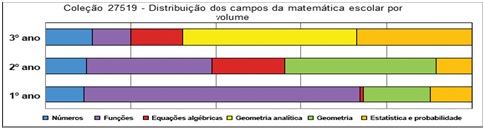
\includegraphics[width=0.5\textwidth]{1}
      \end{figure}

      \item Coleção 27582 - Essa coleção eliminou alguns tópicos dispensáveis nessa fase do ensino, no entanto, ainda há excesso de conteúdo matemático proposto e, por vezes, conceitos indicados como opcionais são empregados posteriormente, criando uma certa inconscistência.
      \begin{figure}[h!]
      \centering
      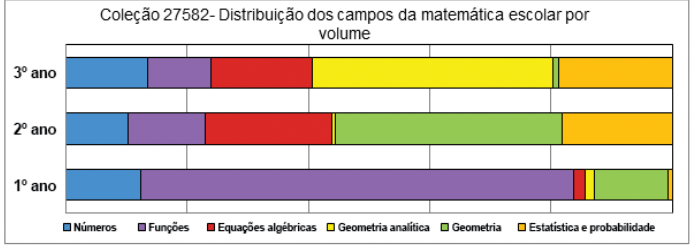
\includegraphics[width=0.5\textwidth]{2}
      \end{figure}

      \item Coleção 27583 - A seleção e organização dos conteúdos matemáticos dessa obra segue o padrão adotado pelas outras, no qual o estudo de funções está concentrado no primeiro volume e o geometria analítica no último volume. Essa abordagem pode prejudicar a inter-relação entre os conteúdos. Não obstante, há um empenho no estabelecimento de articulações entre os conhecimentos novos e os já abordados, o que é um aspecto elogiável da coleção.
      \begin{figure}[h!]
      \centering
      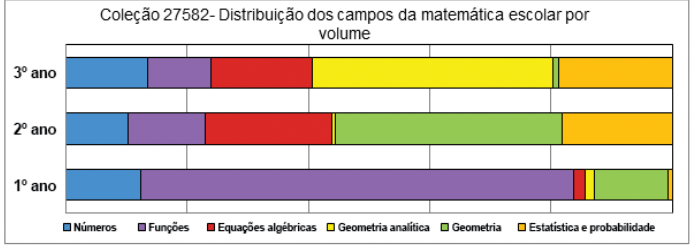
\includegraphics[width=0.5\textwidth]{3}
      \end{figure}

      \item Coleção 27585 - A obra é caracterizada pelo excesso de conteúdos a estudar e pelo seu detalhamento exagerado. O particionamento de funções no primeiro volume, geometria no segundo e geometria analítica no terceiro, acompanha o padrão das outras obras, o que não favorece a conexão entre os conteúdos. Apesar disso, nessa obra os campos dos números e da estatística e probabilidade são dosados satisfatoriamente nos três volumes.
      \begin{figure}[h!]
      \centering
      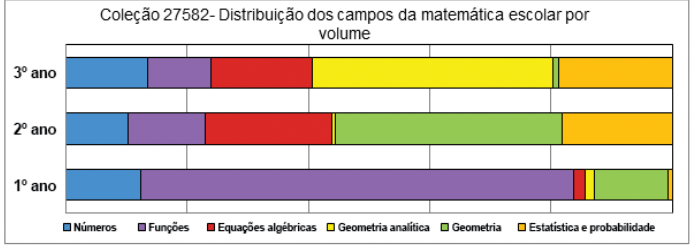
\includegraphics[width=0.5\textwidth]{4}
      \end{figure}

      \item Coleção 27588 - Há uma grande quantidade de conteúdos nessa obra e os conteúdos também não estão bem distribuídos, exceto a trigonometria e as funções trigonométricas que estão presentes nos três volumes.
      \begin{figure}[h!]
      \centering
      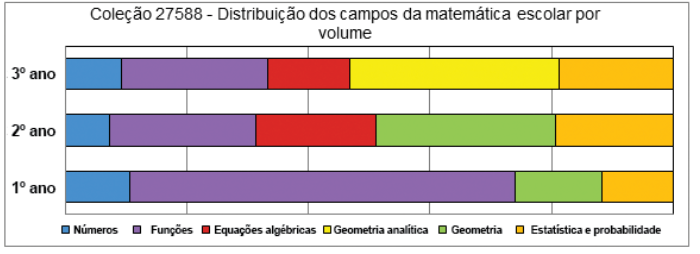
\includegraphics[width=0.5\textwidth]{5}
      \end{figure}

      \item Coleção 27602 - Há opção de limitar as funções trigonométricas do seno e cosseno é uma escolha elogiável. Soma-se a isso, a discussão de alguns tópicos de matemática financeira. No mais, a abordagem é igual das outras obrais, nos quais o estudo de funções é concentrado no primeiro livro e as geometrias no terceiro.
      \begin{figure}[h!]
      \centering
      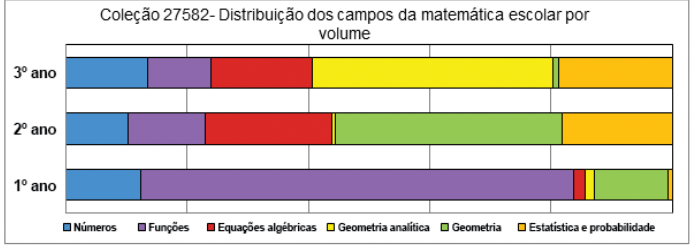
\includegraphics[width=0.5\textwidth]{6}
      \end{figure} 
    \end{enumerate}
  \item Manual do Professor
    \begin{enumerate}
    \item Coleção 27519
      \begin{description}
      \item[Avaliação do Manual do Professor]
        São feitas indicações de leituras significativas que podem, de fato, contribuir para a formação docente. As orientações didáticas são igualmente importantes para o trabalho do professor e bem apoiadas pelas atividades propostas e complementares. \\
        No entanto, o Manual ressente-se de um bom direcionamento de possíveis alterações a serem realizadas na ordem de apresentação dos conteúdos e de quais conteúdos devem ser priorizados.
      \item[Avaliação do professor]
        Analisando a tabela nota-se que o manual do professor dessa obra cumpre com o seu papel, principalmente nas soluções das atividades propostas, das orientações para o desenvolvimento das atividades e as contribuições para formação do professor.
      \end{description}
    \item Coleção 27582
      \begin{description}
      \item[Avaliação do Manual do Professor]
        Os pressupostos teóricos, os objetivos que nortearam a elaboração da coleção e a metodologia adotada estão bem explicitados no Manual. Entretanto, nem sempre as opções metodológicas adequadas são plenamente seguidas no Livro do Aluno. \\
        São apresentados, por capítulo, os conteúdos abordados no texto do aluno com  os  respectivos  objetivos,  habilidades  e  competências  associados  à  matriz  de referência do Enem e considerações sobre algumas das atividades propostas, além de outras, que podem complementar o trabalho em sala de aula.\\
        No manual, encontram-se indicações de sites, softwares, que visam contri-buir para a formação continuada do professor. A bibliografia indicada seria mais útil ao docente caso destacasse os títulos mais importantes e incluísse itens mais atualizados.
      \item[Avaliação do professor]
        De acordo com a tabela do PNLD, o manual do professor dessa coleção é no geral suficiente, exceto nas orientações para avaliação da aprendizagem que é superficial.
      \end{description}
      
    \item Coleção 27583
      \begin{description}
      \item[Avaliação do Manual do Professor]
        Os objetivos que norteiam a elaboração da coleção são claros e coerentes com os pressupostos teóricos expostos na denominada Parte Geral do Manual. São apresentadas reflexões sobre o papel da avaliação e sobre alguns dos aspectos a serem observados  nesse  processo,  além  dos  diferentes  instrumentos  que  podem  ser  utilizados.  Também se discute a importância da análise atenta da produção escrita dos alunos e, ainda, o papel do erro para o aperfeiçoamento dos processos de ensino e de aprendizagem.\\
        Por  outro  lado,  há  poucas  orientações  sobre  possíveis  sequências  de  estudo  dos conteúdos do Livro do Aluno. Apesar disso, o Manual oferece subsídios metodológicos relativos aos infográficos e aos demais tópicos abordados na obra. São também incluídas sugestões de atividades extras para os alunos, como problemas, jogos, leitura de textos, pesquisas, entre outras. Ao lado disso, há sugestões de leituras di-versificadas e úteis para a formação continuada do professor.
      \item[Avaliação do professor]
        De todas as coleções analisadas pelo profissionais que fizeram o PNLD, o manual do professor dessa obra se destaca. Quase todos os critérios são classificados com destaque.
      \end{description}
      
    \item Coleção 27585
      \begin{description}
      \item[Avaliação do Manual do Professor]
        O Manual do Professor contém orientações e sugestões de leitura, que fundamentam  e  norteiam  o  trabalho  docente,  além  de  colaborar  para  sua  formação  continuada. Porém, no que se refere a documentos curriculares oficiais, a bibliografia está  desatualizada.  Existem  propostas  de  avaliação  e  orientações  para  a  utilização adequada dos livros. Os três volumes do Manual sugerem atividades complementares, que podem contribuir para a formação do aluno, por meio do aprofundamento do conteúdo.
      \item[Avaliação do professor]
        Assim como a maioria das coleções, o manual do professor dessa coleção cumpre o seu papel, mas vale destacar que algumas características como as orientações para o uso de recursos didáticos e as orientações para o desenvolvimento de atividades poderiam ter sido abordados menos superficialmente.
      \end{description}
      
    \item Coleção 27588
      \begin{description}
      \item[Avaliação do Manual do Professor]
         As concepções didático-pedagógicas apresentadas no Manual do Professor são compatíveis com as tendências mais atualizadas da Educação Matemática. Contudo, não é plenamente satisfatória a concretização dessas concepções no Livro do Aluno. Na verdade, há excesso de conteúdos propostos, apresentados de modo demasiadamente detalhado e compartimentado. Também foi observado que, nas explanações, não são feitos questionamentos que incentivem o aluno a participar mais autonomamente do processo de aprendizagem. \\
        Há sugestões apropriadas sobre o que avaliar em cada unidade e, ainda, observações de caráter geral sobre avaliação. A leitura e produção de textos é incentivada. A  resolução  de  boa  parte  dos  exercícios  é  apresentada,  mas  há  poucas  atividades complementares sugeridas e, em vários momentos, sente-se falta de orientações específicas para o desenvolvimento das atividades.
      \item[Avaliação do professor]
        Entre todas as obras analisadas no PNLD, essa apresenta o pior manual do professor de acordo com a sua tabela. Poucos itens são classificados com suficiente e o resto são todos classificados com superficial.
      \end{description}
      
    \item Coleção 27602
      \begin{description}
      \item[Avaliação do Manual do Professor] 
        No Manual, nas orientações específicas por capítulo, há sugestões de questionamentos que podem ser feitos com os alunos sobre as atividades propostas, bem como indicações de sites e textos complementares. \\
        Há, também, sugestão para que o professor selecione ou reordene os conteú dos trabalhados, mas não há orientações suficientes para isso. \\
        São  encontradas  sugestões  para  que  o  docente  faça  atividades  adicionais de pesquisas,  de  uso  de  materiais  e  de  jogos,  bem  como  para  o  desenvolvimento  de projetos  e  experimentos.  Porém,  tais  sugestões  são  genéricas  e  há  poucas  dessas atividades efetivamente elaboradas no Manual.\\
        As  resoluções  das  atividades  estão  presentes  mas,  para  muitas  das  questões objetivas, há somente respostas, sem quaisquer comentários.
      \item[Avaliação do professor]
        O manual do professor dessa obra cumpre com o seu papel, pois praticamente todos os itens de classificação da tabela estão marcados como abordados suficientemente.
      \end{description}
      
    \end{enumerate}
  \end{enumerate}


\end{document}
